\documentclass[11pt, letterpaper]{memoir}
\usepackage{HomeworkStyle}
\geometry{margin=0.75in}



\begin{document}

	\begin{center}
		{\large Quiz 10.2 -- Applications of Symmetry and Group Theory}
	\end{center}
	{\large Name: \rule[-1mm]{4in}{.1pt} 

\subsection*{Irreducible Representations}
Consider the ammonia molecule, which belongs to the $C_{3v}$ symmetry point group. Below are figures showing the molecular orbitals and normal modes of ammonia. Assign each feature to the correct irreducible representation of the $C_{3v}$ point group.

\hspace{-4em}\noindent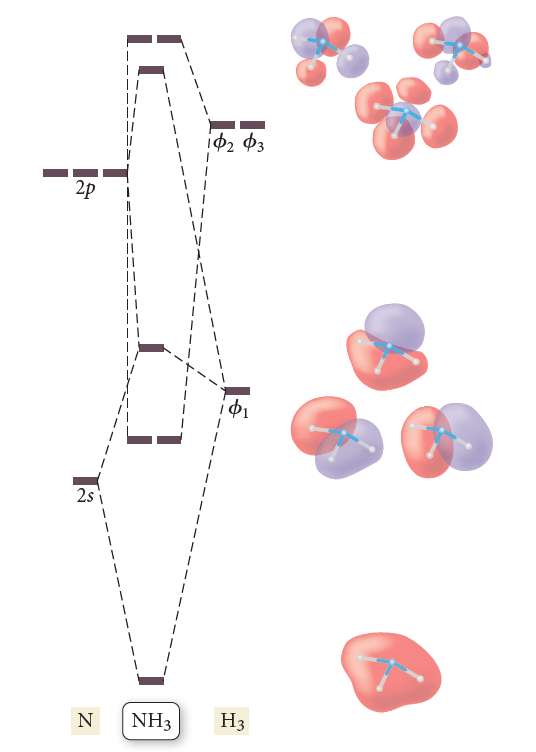
\includegraphics[width=0.5\linewidth]{AmmoniaMOs}
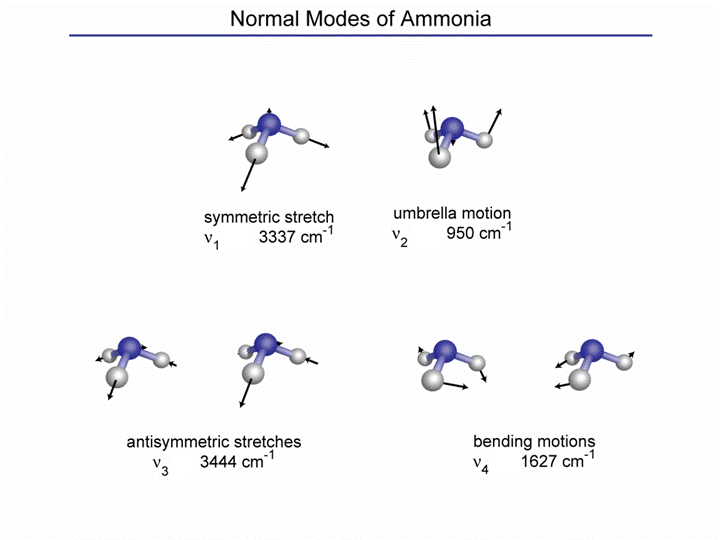
\includegraphics[width=0.6\linewidth]{AmmoniaModes}

\noindent
Which (if any) of the vibrational modes are ``silent'' in IR or Raman spectra

\vspace{6em}\noindent
Is the HOMO-LUMO transition allowed by symmetry? If so, what direction of light polarization can induce the transition?
\end{document}
